% bare_jrnl_compsoc, texV1.4b, 2015/08/26, Michael Shell
\documentclass[10pt,journal,compsoc]{IEEEtran}

% *** MISC UTILITY PACKAGES ***

\newcommand{\note}[1]{\textcolor{magenta}{#1}} 
\usepackage[nocompress]{cite}
\usepackage[]{footmisc}
\usepackage{hyperref} % autoref
% *** GRAPHICS RELATED PACKAGES ***
\ifCLASSINFOpdf
   \usepackage[pdftex]{graphicx}
  % declare the path(s) where your graphic files are
   \graphicspath{{./figures/}}
  % and their extensions so you won't have to specify these with
  % every instance of \includegraphics
  % \DeclareGraphicsExtensions{.pdf,.jpeg,.png}
\else
  % or other class option (dvipsone, dvipdf, if not using dvips). graphicx
  % will default to the driver specified in the system graphics.cfg if no
  % driver is specified.
   \usepackage[dvips]{graphicx}
  % declare the path(s) where your graphic files are
   \graphicspath{{./figures/}}
  % and their extensions so you won't have to specify these with
  % every instance of \includegraphics
   \DeclareGraphicsExtensions{.eps}
\fi

% latex, and pdflatex in dvi mode, support graphics in encapsulated
% postscript (.eps) format. pdflatex in pdf mode supports graphics
% in .pdf, .jpeg, .png and .mps (metapost) formats. Users should ensure
% that all non-photo figures use a vector format (.eps, .pdf, .mps) and
% not a bitmapped formats (.jpeg, .png). The IEEE frowns on bitmapped formats
% which can result in "jaggedy"/blurry rendering of lines and letters as
% well as large increases in file sizes.

% *** MATH PACKAGES ***
%% with other math-related packages, you may want to disable it.
\usepackage{amsmath, amsthm, amsfonts,amssymb,eulervm,xspace, mathtools}
\usepackage{mathrsfs} % math script fonts
\theoremstyle{definition}
\newtheorem{definition}{Definition}[section]
\theoremstyle{remark}
\newtheorem{example}{Example}[section]
% *** SPECIALIZED LIST PACKAGES ***
\usepackage{xcolor}
\usepackage{algorithmic}
\usepackage[utf8]{inputenc}
\usepackage{subfig} %ieee does not like subfigure
\usepackage{multicol}
\usepackage{tikz}
\usetikzlibrary{cd} % commutative diagrams
\newtheorem{prop}{Proposition} %math?
\usepackage[switch]{lineno}
\usepackage{minted}
\setminted[python]{fontsize=\scriptsize, 
                   linenos,
                   numbersep=8pt,
                   autogobble, 
                   frame=lines,
                   framesep=3mm} 
% *** ALIGNMENT PACKAGES ***
\usepackage{array}
\usepackage{tabulary}
% IEEEtran contains the IEEEeqnarray family of commands

% *** SUBFIGURE PACKAGES ***
\ifCLASSOPTIONcompsoc
  \usepackage[caption=false,font=footnotesize,labelfont=sf,textfont=sf]{subfig}
\else
  \usepackage[caption=false,font=footnotesize]{subfig}
\fi

% *** FLOAT PACKAGES ***
\usepackage{dblfloatfix}

% *** PDF, URL AND HYPERLINK PACKAGES ***
\usepackage{url}

% *** Do not adjust lengths that control margins, column widths, etc. ***
% *** Do not use packages that alter fonts (such as pslatex).         ***
% There should be no need to do such things with IEEEtran.cls V1.6 and later.
% (Unless specifically asked to do so by the journal or conference you plan
% to submit to, of course. )

\usepackage{notation} %notation conventions
% correct bad hyphenation here
\hyphenation{op-tical net-works semi-conduc-tor}


\begin{document}
%
\title{Topological Equivariant Artist Model for Visualization Library Architecture}
% author names and IEEE memberships
\author{Hannah~Aizenman, Thomas~Caswell, and~Michael~Grossberg,~\IEEEmembership{Member,~IEEE,}% <-this % stops a space
\IEEEcompsocitemizethanks{\IEEEcompsocthanksitem H. Aizenman and M. Grossberg are with the department of Computer Science, City College of New York. 
\protect\\
% note need leading \protect in front of \\ to get a newline within \thanks as
% \\ is fragile and will error, could use \hfil\break instead.
E-mail: haizenman@ccny.cuny.edu, mgrossberg@ccny.cuny.edu 
\IEEEcompsocthanksitem Thomas Caswell is with National Synchrotron Light Source II, Brookhaven National Lab 
\protect \\
E-mail: tcaswell@bnl.gov}% <-this % stops an unwanted space
\thanks{Manuscript received X XX, XXXX; revised X XX, XXXX.}
}


% for Computer Society papers, we must declare the abstract and index terms
% PRIOR to the title within the \IEEEtitleabstractindextext IEEEtran
% command as these need to go into the title area created by \maketitle.
% As a general rule, do not put math, special symbols or citations
% in the abstract or keywords.
\IEEEtitleabstractindextext{%
\begin{abstract}
The abstract goes here.
\end{abstract}

% Note that keywords are not normally used for peerreview papers.
\begin{IEEEkeywords}
%Computer Society, IEEE, IEEEtran, journal, \LaTeX, paper, template.
\end{IEEEkeywords}}


% make the title area
\maketitle


\IEEEpeerreviewmaketitle



\IEEEraisesectionheading{\section{Introduction}\label{sec:introduction}}


\IEEEPARstart{T}his paper uses methods from algebraic topology and category theory to develop a model of the transformation from data to graphical representation. This model provides a language to specify how data is structured and how this structure is carried through in the visualization, and serves as the basis for a functional approach to implementing visualization library components. Topology allows us to describe the structure of the data and graphics in a generalizable, scalable, and trackable way. Category theory provides a framework for separating the transformations implemented by visualization libraries from the various stages of visualization and therefore can be used to describe the constraints imposed on the library components \cite{wielsManagementEvolvingSpecifications1998,goguenCategoricalManifesto1991}. Well constrained modular components are inherently functional\cite{hughesWhyFunctionalProgramming1989}, and a functional framework yields a library implementation that is likely to be shorter, clearer, and more suited to distributed, concurrent, and on demand tasks\cite{huHowFunctionalProgramming2015}. Using this functional approach, this paper contributes a practical framework for decoupling data processing from visualization generation in a way that allows for modular visualization components that are applicable to a variety of data sets in different formats. \note{is it OK that this is something reviewer 4 wrote}



\section{Related Work}
This work aims to develop a model for describing visualization transformations that can serve as guidance for how to architecture a general purpose visualization library. We define a general purpose visualization library as one that provides non domain specific building block components\cite{wongsuphasawatNavigatingWideWorld2021} for building visualizations, for example functions for converting data to color or encoding data as dots. In this section, we describe how visualization libraries attempt this goal and discuss work that formally describes what properties of data should be preserved in a visualization. We restrict the properties of data that should be preserved to 

\begin{LaTeXdescription}
  \item [continuity] how elements in a dataset are organized, e.g. discrete rows in a table, networked nodes, pixels in an image, points on a line
  \item [equivariance] functions on data that have an equivalent effect on the graphical representation, e.g. rotating a matrix has a matching rotation of the image, translating the points on a line has a matching visual shift in the line plot
\end{LaTeXdescription}

\subsection{Continuity}
\begin{figure}[!h]
  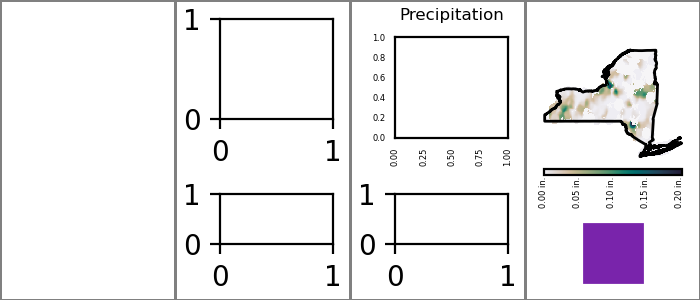
\includegraphics[width=\columnwidth]{k_different_types.png}
  \caption{Continuity is how elements in a data set are connected to each other, which is distinct from how the data is structured. The rows in (a) are discrete, therefore they have discrete continuity as illustrated by the discrete dots. The gaussian in (b) is a 1D continuous function, therefore the continuity of the elements of the gaussian can be represented as a line on an interval (0,1). In (c), every element of the globe is connected to its nearest neighbors, which yields a 2D continuous continuity as illustrated by the square.}
  \label{fig:related-work:continuity}
\end{figure}
Continuity describes elements in a data set are organized; this concept is termed topological properties by Wilkinson\cite{wilkinsonGrammarGraphics2005}. Wilkinson provides the examples of values that are isolated from each other, and therefore discrete, and values lying on a continuum or in a compact region. For example, in \autoref{fig:related-work:continuity}, each station record in the table is independent of the others; therefore, the continuity of the table is discrete. The data provided by the gaussian are points sampled along the curve, therefore the continuity of the points on the line is 1D continuous. Every point on the globe is connected to its 6 nearest cardinal neighboring points (NW, N, NE, E, SE, S, SW, W). We propose that a robust model of continuity provides a way to develop library components that can work on the data in small pieces in a manner where the overall continuity of the data is preserved in the visual transformation. 

\begin{figure}[!h]
  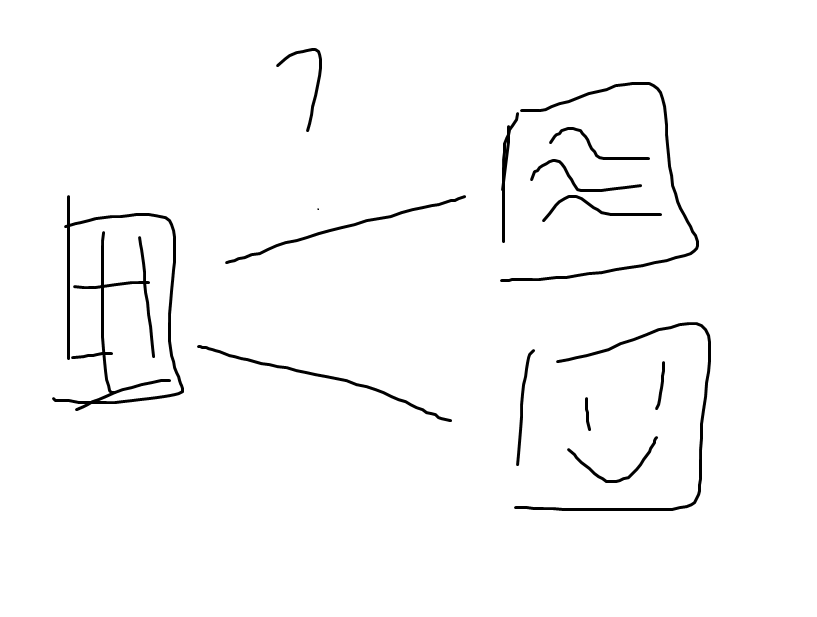
\includegraphics[width=\columnwidth]{whycontinuity.png}
  \caption{Continuity is implicit in choice of visualization rather than explicitly in choice of data container. The line plots in (b) are generated by a 2D table (a). Structurally this table can be identical to the 2D matrix (a) that generates the image in (c).}
  \label{fig:related-work:visual-algorithm}
\end{figure}

 The preservation of continuity can be made explicit, as in the transformation of table to parallel coordinates in Ruchikachorn and Mueller \cite{ruchikachornLearningVisualizationsAnalogy2015}, but is often expressed implicitly in the choice of visual algorithm (visualization type), as explored in taxonomies by Tory and M\"{o}ller \cite{toryRethinkingVisualizationHighlevel2004} and Chi\cite{chiTaxonomyVisualizationTechniques2000}.

For example, in \autoref{fig:related-work:visual-algorithm} the same table can be interpreted as a set of 1D continuous curves when visualized as a collection of line plots or as a 2D surface when visualized as an image.  This means that often there is no way to express data continuity independent of visualization type, meaning most visualization libraries will allow, for example, visualizing discrete data as a line plot or an image. General purpose visualization libraries-such as Matplotlib\cite{hunterMatplotlib2DGraphics2007}, Vtk\cite{hanwellVisualizationToolkitVTK2015,geveciVTK2012}, and D3 \cite{bostockDataDrivenDocuments2011}-carry distinct data models as part of the implementation of each visual algorithm. The lack of unified data model means that each plot in a linked\cite{beckerBrushingScatterplots1987,bujaInteractiveData1991} visualization is treated as independent, as are the transforms converting each field in the data to a visual equivalent.

Domain specific libraries can often guarantee consistency because they have a single model of the data in their software design, as discussed in Heer and Agarwal \cite{HeerSoftware2006}'s survey of visualization software design patterns. For example, the relational database is core to tools influenced by APT, such as Tableau\cite{StoltePolaris2002,hanrahanVizQL2006,MackinlayShowme2007} and the Grammar of Graphics\cite{wilkinsonGrammarGraphics2005} inspired ggplot\cite{wickhamGgplot2ElegantGraphics2016a}, Vega\cite{satyanarayanDeclarativeInteractionDesign2014} and Altair\cite{vanderplasAltairInteractiveStatistical2018}. Images underpin scientific visualization tools such as Napari\cite{nicholas_sofroniew_2021_4533308} and ImageJ\cite{schneiderNIHImageImageJ2012} and the digital humanities oriented ImagePlot\cite{studiesCulturevisImageplot2021} macro; the need to visualize and manipulate graphs has spawned tools like Gephi\cite{bastianGephiOpenSource2009}, Graphviz\cite{ellsonGraphvizOpenSource2002}, and Networkx\cite{HagbergExploringNetwork2008}. 
 
\subsubsection{Fiber Bundles}
\label{sec:related-work:fiber-bundles}
\begin{figure}[h!]
  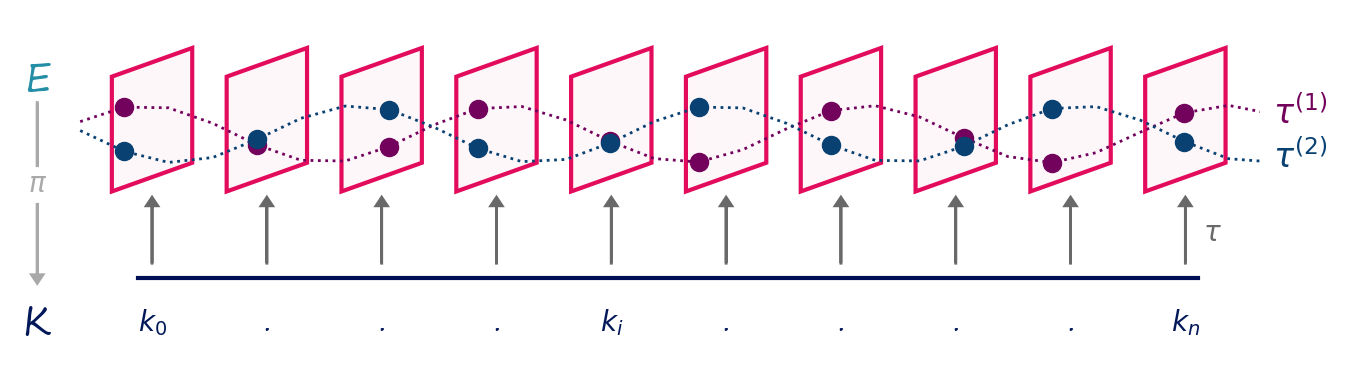
\includegraphics[width=\columnwidth]{fiberbundle.png}
  \caption{A fiber bundle is mathematical construct that allows us to express the relationship between data and continuity. The \textcolor{total}{total} space \dtotal is the topological space in which the data is embedded. The \textcolor{fiber}{fiber} space \dfiber\ is embedded in \dtotal\ and is the set of all possible values that any
  \note{add big rectangle E}}
  \label{fig:related-work:fiber-bundle}
\end{figure}

The model described in this work provides a model for expressing data sets with different topological properties. 
We obtain this generality by using a mathematical structure called a fiber bundles as the basis of our abstraction, as proposed by Butler, Bryson, and Pendley\cite{butlerVisualizationModelBased1989,
butlerVectorBundleClassesForm1992}. As described by them, a fiber bundle is a formal model of the mapping between data points and the underlying topological space they lie in. For example, nodes on a network and the graph of the network, an image and the underlying grid at which the image is sampled, or table columns and the table index.

Formally, a fiber bundle is a mathematical structure $(\dtotalc, \dbasec, \pi, \dfiberc)$
\begin{equation}
  \label{eq:fiber_bundle}
  \begin{tikzcd}
      \dfiberc \arrow[r, hook] & \dtotalc \arrow[r, "\pi"] & \dbasec
  \end{tikzcd}
\end{equation}

\begin{definition}
The \textcolor{base}{base space} \dbasec\ is a topological space, which means it is a set $\dbase$ with a collection of open sets \cite{TopologyVsTopology} surrounding each element in the set. Open sets are a collection of subsets $\{\opensetc\}$ in a set \dbase, including the empty set, the whole set \dbase, and every union and intersection of its member subsets. For each point $\dbasepoint \in \dbase$, there is a collection of subsets $\\{\openset\} \subset \dbase$ such that $\dbasepoint \in \openset \subseteq \dbase$ \cite{spanier1989algebraic, bradleyTopologyCategoricalApproach2020}  
\end{definition}
\note{intuition about base space}

\begin{definition} The \textcolor{fiber}{fiber space} \dfiberc\ is a topological space such that for every $\dbasepoint \in \dbase$, the fiber over that point is isomorphic to the preimage of that point $\dfiber_{\dbasepoint} \cong \pi^{-1}(\{\dbasepoint\})$. All fibers $\dfiber_{\dbasepoint}$ are homeomorphic to each other \cite{spanier1989algebraic, hatcherAlgebraicTopology2002}
\end{definition}
\note{intuition about fiber} 

\begin{definition} The \textcolor{total}{total space} \dtotalc\ is the space reachable via the projection map $\pi$. The total space is always locally trivial, meaning $\dtotal = \dbase \times \dfiber$ over any open neighborhood $\openset_{\dbasepoint}$. 
\end{definition}
The fiber bundle is trivial when $\dtotal = \dbase \times \dfiber$ is true globally; a non-trivial bundle can be thought of as the twisted fiber product $\dtotal=\dbase times_{T} \dfiber$\cite{hatcherAlgebraicTopology2002,nlab:twisting_function}. The twisting refers to the fiber \dfiber\ not aligning in the same direction over all $\dopenspace \subseteq \dbase$. 

\begin{equation}
  \begin{tikzcd}
      \dfiberc \arrow[r, hook] & \dtotalc \arrow[d, "\pi"'] \\
                        & \dbasec \arrow[u, "\dsectionc"', bend right]
  \end{tikzcd}
\end{equation}

How these spaces fit together is illustrated in \autoref{fig:related-work:fiber-bundle}, wherein values lives in the fiber $\dfiber\subseteq\dtotal$. In this example, the fiber \dfiber\ is the cartesian product of two sets $F_{0}\times F_{1}$ where each fiber $F_{i}$ is ....

\subsubsection{Sheaves}
The set of all sections sections $\{\dsection^{i}: \openset_{j}\rightarrow \dtotal\}|_{i\in I}$ over an arbitrary open set $U_{j}$ is denoted $\Gamma(\openset_{\dbasepoint}, \dtotal)$. The set of all sections over the total space \dbase\ is denoted $\Gamma(\dbase, \dtotal)$.  

The map from the open set to the set of sections is called a presheaf $\sheaf: U_j \rightarrow \Gamma(\openset_j, \dtotal)$ \cite{spanier1989algebraic,SheafMathematics2021,nlab:presheaf}. The presheaf preserves inclusion maps between the open sets open sets $\iota$ and the inclusion map $\iota^*$ between the sets of sections.

\begin{equation}
  \label{eq:related-work:continuity:presheaf}
  \begin{tikzcd}[column sep=small]
    {\Gamma(\opensetc_1, \dtotalc)}                                       & {}                                                    & {\Gamma(\opensetc_2, \dtotalc)} \arrow[ll, "\iota^*"', hook'] \\
                                                                  &                                                       &                                                       \\
    \opensetc_1 \arrow[uu, "\sheafc_{\dtotal}"] \arrow[rr, "\iota"', hook] & {} \arrow[uu, "\sheafc_{\dtotal}" description, dotted] & \opensetc_2 \arrow[uu, "\sheafc_\dtotal"']                    
    \end{tikzcd}
\end{equation}

This means that a smaller space $\openset_1$ is included in a larger space $\openset_2$ and a function that is continuous over a larger space $\openset_2$ is continuous over a subspace $\openset_1 \subspace \openset_2$. Sheaves are presheafs where sets of sections $\Gamma$ are defined over unions of open sets over a topology $\bigcup_{j \in I} \openset)_j \in \dtotal$ \cite{spanier1989algebraic, nlab:sheaf}. Sheaves are often used as an abstraction for keeping track of how data over topological spaces is glued together \cite{ghristElementaryAppliedTopology2014} because they model the data as sets of sections, continuity of the data in the base, and how subsets fit together through inclusion maps.  

\note{I've seen this convention before, but I also cite all these people above}
For more information on fiber bundles and sheaves, see Hatcher\cite{hatcherAlgebraicTopology2002}, Munkres\cite{munkresElementsAlgebraicTopology1984}, Spanier \cite{spanier1989algebraic} and Ghrist\cite{ghristElementaryAppliedTopology2014,ghristHomologicalAlgebraData2018}. 

\subsection{Equivariance}
\label{sec:related-work:equivariance}
When introducing the retinal variables, Bertin informally specifies that continuity is preserved in the mark and defines equivariance constraints in terms of data and visual variables being selective, associative, ordered, or quantitative\cite{bertinSemiologyGraphicsDiagrams2011a}. In the \textit{A Presentation Tool}(APT) model, Mackinlay embeds the continuity constraint in the choice of visualization type and generalizes the equivariance constraint to preserving a binary operator from one domain to another. The algebraic model of visualization\cite{kindlmannAlgebraicProcessVisualization2014}, proposed by Kindlmann and Scheidegger, restricts equivariance to invertible transformations.

\begin{figure}[!h]
  \label{fig:related-work:equivariance}
  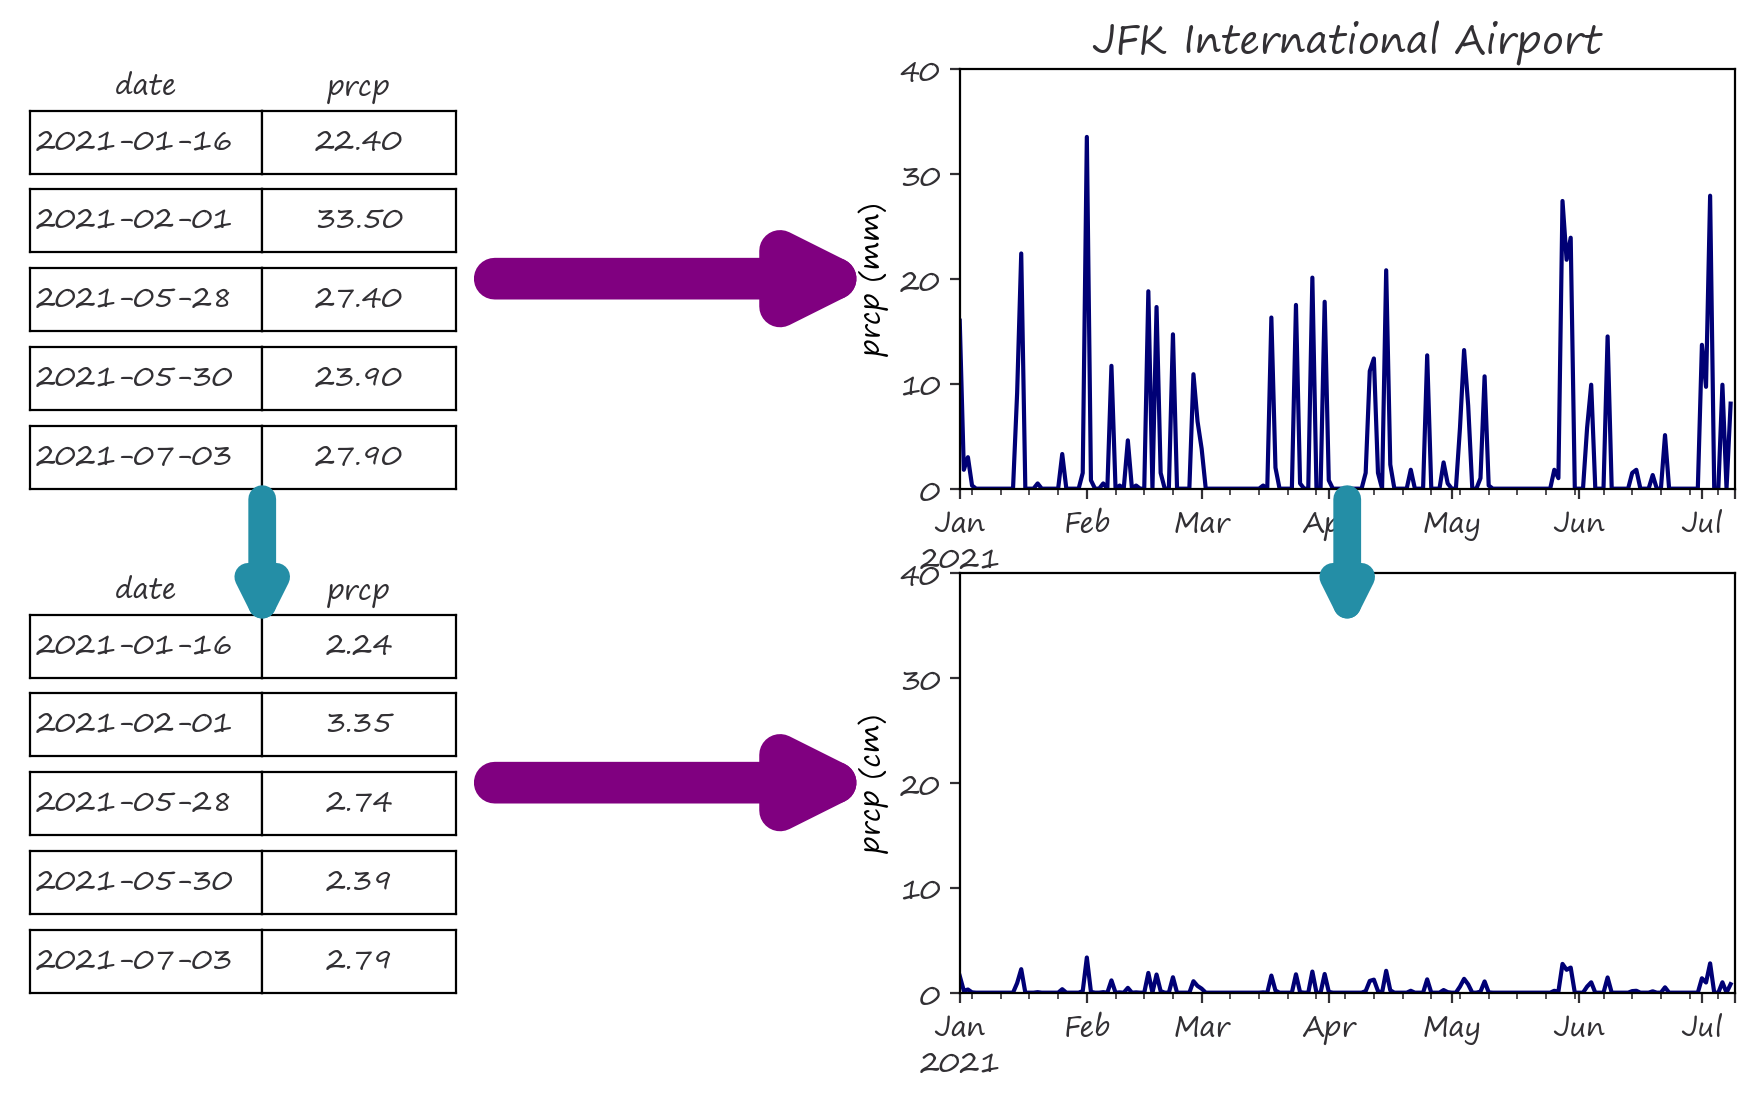
\includegraphics[width=\columnwidth]{equiv.png}
  \caption{Equivariance is that a transformation on the data has a corresponding transformation in the graphical representation. For example, in this figure the data is scaled by a factor 10. Equivalently the line plot is scaled by factor of 10, resulting in a shrunken line plot. Either a transformation on the data side can induce a transformation on the visual side, or a transformation on the visual side indicates that there is also a transformation on the data side. }
\end{figure}

\subsubsection{Category Theory}
\label{sec:related-work:equivariance:category}
In this work, we propose that equivariance constraints can be expressed using category theory. Vickers et. al \cite{vickersUnderstandingVisualizationFormal2013} provide a brief introduction to category theory for visualization practitioners, but their work focuses on reasoning about visualization design, while this paper aims to provide guidance on designing visualization library components. Briefly we introduce concepts in category theory that we use to describe our model in \autoref{sec:artist:category} and \autoref{sec:artist:construction}. 

\note{the notation here may need to be X and Y}

\begin{definition} A category \mathcal{C} consists of a collection of objects $C$ with identity $id_c: C\rightarrow C$ and the set of morphisms between every two objects $f:C_1 \rightarrow C_2$, \cite{fongInvitationAppliedCategory2019,maclaneCategoriesWorkingMathematician2013}. 
\end{definition}
The set of morphisms between objects is termed the hom set $hom_{\mathcal{C}}(C_1, C_2)$. The morphisms on the category  compose
\begin{equation*}
  \begin{tikzcd}
    C_1 \arrow[r, "f"] \arrow[rd, "g\circ f"'] \arrow["id_{C_1}"', loop, distance=2em, in=215, out=145] & C_2 \arrow[d, "g"] \arrow["id_{C_2}"', loop, distance=2em, in=125, out=55] \\
  & C_3 \arrow["id_{C_3}"', loop, distance=2em, in=305, out=235]              
  \end{tikzcd}
\end{equation*}
 and are constructed such that the following axioms hold \cite{riehlCategoryTheoryContext}:
 \begin{LaTeXdescription}
   \item[associativity] if $f: C_1 \rightarrow C_2$, $g: C_2 \rightarrow C_3$ and $h: C_3 \rightarrow C_4$ then $h\circ (g \circ f) = (h \circ g) \circ f$
   \item[identity] for every $f: C_1 \rightarrow C_2$ there exists identity morphisms $f \circ id_{C_1} = f = id_{C_2} \circ f$
 \end{LaTeXdescription}

 \begin{definition} An opposite category $\mathcal{C}^{op}$ is a category with all the same objects of category $\mathcal{C}$ and but the morphisms are reversed. For example $f:C_1 \rightarrow C_2$ in $\mathcal{C}$ is $f:C_2 \rightarrow C_1$ in $\mathcal{C}^{op}$.   
 \end{definition}

 \begin{definition} A functor is a morphism between categories $\mathfrak{F}: \mathcal{C} \rightarrow \mathcal{D}$. A functor has the properties of identity and composition \cite{riehlCategoryTheoryContext}\end{definition}
A functor preserves the structure of the category, namely morphisms and the source and target objects of those morphisms, composition of morphisms, and identity morphisms \cite{riehlCategoryTheoryContext}. Contravariant functors are functors where the morphisms in $\mathcal{C}$ go in the opposite direction from the morphisms in $\mathcal{D}$.  

 \begin{definition} A presheaf \sheafc\, as introduced in \autoref{eq:related-work:continuity:presheaf}, is a functor $\sheaf: \mathcal{C}^{op} \rightarrow \textbf{Set}$.\cite{nlab:presheaf} \end{definition}

 \begin{definition} A natural transformation is a morphism of functors $\alpha: F \rightarrow G$ where $F, G$ are functors from $\mathcal{C}$ to $\mathcal{D}$. \cite{riehlCategoryTheoryContext, bradleyWhatNaturalTransformation}
 \end{definition}
The natural transformation acts as a wrapper of sorts
\begin{equation}
  \label{eq:related-work:equivariance:natural-transform}
\begin{tikzcd}
  & {} \arrow[dd, "\alpha", Rightarrow, shorten=1.5em] &             \\
\mathcal{C} \arrow[rr, "F", bend left] \arrow[rr, "G"', bend right] &                                     & \mathcal{D} \\
  & {}                                  &            
\end{tikzcd}
\end{equation}
such that $\alpha(F: \mathcal{C} \rightarrow \mathcal{D}) = G: \mathcal{C} \rightarrow \mathcal{D}$ commutes for any morphism $f:c\rightarrow c^{\prime}$ \cite{fongInvitationAppliedCategory2019}. Arbitrary morphisms on sheaves are natural transforms \cite{SheafMathematics2021,bradleyWhatNaturalTransformation}. 

For more information on category theory, see Barr and Wells\cite{barrCategoryTheoryComputing}, Fong and Spivak \cite{fongInvitationAppliedCategory2019}, Riehl\cite{riehlCategoryTheoryContext} and Bradley et. al. \cite{bradleyTopologyCategoricalApproach2020}.

\section{Artist} 
In this section, we use category theory to formally express the implicit assumptions that visualization library components make in transforming data into graphical representations. We propose that the visualization transformation can be modeled as a functor, which we call the \textcolor{artist}{Artist} \vartist \footnote{We call this transformation the artist because the \mintinline{python}{Artist} object in Matplotlib\cite{hunterMatplotlib2DGraphics2007}}. The artist \vartist\ converts data, which we model as the sheaf $\sheafc_{\dtotalc}$ to graphics in the sheaf $\sheafc_{\gtotalc}$. We formulate this association as 

\begin{equation}
  \label{eq:artist:artist}
  \vartistc: \sheafc_{\dtotalc} \rightarrow \sheafc_{\gtotal}
\end{equation}

In this section we describe the structure of the data and graphic spaces, which we formulate as objects in categories and the morphisms between those objects. We then use these definitions to express the structure that an artist must preserve. Finally, we propose that artists can be composed by manufacturing new artists based on various types of input data. 

\subsection{Categorical Artist}
\label{sec:artist:category}

Fiber bundles, as introduced in \autoref{sec:related-work:fiber-bundles}, serve as the model of data and graphic spaces in out model. In this section, we introduce categorical formulations of the topological spaces that make up a fiber bundle. 

We introduce the category $\mathcal{\dbase}$ to encapsulate the subsets of the continuity and the inclusion maps that glue them together. 

\begin{definition} \label{def:category:K} The category of open sets $\mathcal{\dbasec}$ consists of
  \begin{itemize}
    \item \textit{objects} open sets $\openset_{j} \in \{openset\}$ in the topological space $(\dbase, \mathscr{T})$), including the empty set $\varnothing$ and the maximum set \dbase. 
    \item \textit{morphisms} $\iota: U_{j} \hookrightarrow U_{k}$ for all  $U_j, U_k \subset \dtotal$
  \end{itemize} 
\end{definition}

\begin{definition} \label{def:category:E} The category \mathcal{\dtotalc} is a subcategory of \textbf{Set} and consists of 
  \begin{itemize}
    \item \textit{objects} sets of sections $\Gamma(\openset_{j}, \dtotal)$ for all $U_j \subset \dtotal$
    \item \textit{morphisms}  $\iota^*: \Gamma(\openset_{k}, \dtotal) \hookrightarrow \Gamma(\openset_{j}, \dtotal)$ for all  $\openset_j, \openset_k \subset \dtotal$
  \end{itemize} 
\end{definition}


We model data as the sheaf $\sheafc_{\dtotalc}: \mathcal{\dbasec}^{op}\rightarrow \mathcal{\dtotalc}$
\begin{equation}
  \label{eq:artist:morphism-of-sheaf-data}
  \begin{tikzcd}
    & \mathcal{\dtotalc} & \\
{} \arrow[rr, "\dfuncc", Rightarrow, shift right, shorten=3em] & & {} \\
    & \mathcal{\dbasec}^{op} \arrow[uu, "\sheafc_{\dtotalc}", bend left] \arrow[uu, "\sheafc_{\dtotalc}"', bend right] &   
\end{tikzcd}
\end{equation}
where the map \dfunc\ is any arbitrary function between sheafs. The sheaf $\sheaf_{\dtotal}$ over a limit of open sets that contain a point $\dbasepoint \in \dbase$ is approximately the same as a sheaf over a point \dbasepoint\ and is called the stalk $\sheaf_{\mathcal{\dtotal}}|_{k}\coloneqq \lim\limits_{U\ni k} \Gamma(U, \dtotal)$ \cite{StalkSheaf2019}. 

\begin{definition} 
  \label{def:category:F} 
  The fiber category $\mathcal{\dfiberc}$ is a product category\cite{maclaneCategoriesWorkingMathematician2013,nlab:product_category} of zero or more arbitrary categories. In the two category case, the category $\mathcal{\dfiberc}$ consists of 
  \begin{itemize}
    \item \textit{objects} ordered pairs $(x,y)$,  $x$ is an object of $\mathcal{X}$ and  $y$ is an object of $\mathcal{Y}$
    \item \textit{morphisms} ordered pairs $(f:x\rightarrow x^{\prime}, g:y\rightarrow y^{\prime})$
    \end{itemize}
The coomposition of morphisms is defined component wise by composition in $\mathcal{X}$ and $\mathcal{Y}$.ss
\end{definition}

The fiber space over a point is embedded in the stalk over that point $\dfiber_{\dbasepoint}\hookrightarrow \mathscr{\dfiber}_{\dbasepoint}$. The sheaf maps \dfunc\ restricted to the stalk are members of $hom_{\mathcal{\dfiber}}(\dfiber,\dfiber)$. The maps $\varphi \in Hom_{\mathcal{\dfiber}}(\dfiber,\dfiber)$ include the types of data transformations described in \autoref{sec:related-work:equivariance}. When a fiber bundle is trivial, we can dispense with localization and directly consider the fiber maps $Hom(\dfiber_{\dbasepoint}, \dfiber_{\dbasepoint})$ over a point \dbasepoint. In \autoref{sec:artist:construction}, we assume that the fiber bundles are trivial.

The domain of the artist function is the space of all possible graphics. As with the domain $\sheaf_{E}$, the grapic space is modeled with fiber bundle equivalent categories:
\begin{table}[!h]
  \centering
  \label{tab:artist:graphic}
  \begin{tabular}{l l l}
    fiber bundle & data & graphic \\
    \textcolor{base}{base space} & \mathcal{\dbasec} & \mathcal{\gbasec}\\
    \textcolor{total}{total space} & \mathcal{\dtotalc} & \mathcal{\gtotalc}\\
    \textcolor{fiber}{fiber space} & \mathcal{\dfiberc} & \mathcal{\gfiberc}\\
    \pi^{-1} & \sheaf_{\mathcal{\dtotalc}} & \sheaf_{\mathcal{\gtotalc}}\\
  \end{tabular}
\end{table}

The category $\mathcal{H}$ has as objects the sets of functions that generate every arbitrary graphic over the open sets in $\mathcal{\gtotal}$. While $\mathcal{H}$ is the domain of the artist \vartist, the range of \vartist\ is the subset of graphics $\sheaf_{\vartist} \subset \sheaf_{\mathcal{\dtotal}}$ such that structure imposed by $\dfunc_{\dtotal}$ commutes 
\begin{equation}
  \label{eq:artist:equivariance}
  \begin{tikzcd}
    \sheafc_{\dtotalc} \arrow[r, "\vartistc"] \arrow[d, "\dfuncc_{\dtotalc}"'] & \sheafc_{\vartistc} \arrow[d, "\dfuncc_{\vartistc}"] \\
    \sheafc_{\dtotalc} \arrow[r, "\vartistc"] & \sheafc_{\vartistc}                                              
  \end{tikzcd}
\end{equation}
The equivariance condition expressed in \autoref{eq:artist:equivariance} is that a graphic generated by  transforming and then visualizing data $\vartist(\dfunc_{\dtotal}(\sheaf_{\mathcal{dtotal}}))$ can equivalently be generated by visualizing the data and then transforming the graphic $\dfunc_{\vartist}(\vartist(\sheaf_{\mathcal{\dtotal}}))$. This is a formal statement of the equivariance illustrated in \autoref{fig:related-work:equivariance}

In \autoref{sec:artist:construction}, we show a method of constructing the artist such that the constraints of \autoref{eq:artist:morphism-of-sheaf} and \autoref{eq:artist:equivariance} can be satisfied, thereby ensuring equivariance and the preservation of continuity. We then use this formulation to guide the development of visualization library components in \autoref{sec:case-study}.

\subsection{Composition of Artists}
\label{sec:artist:union}
Visualizations generally consist of more than one visual element, for example line plots, a legend, axis ticks, spines, and labels.  We propose that we can express expected consistency between these elements as a preservation of morphisms between objects of different data categories $\mathcal{\dtotal}$. 


\subsubsection{Shared Index}
\begin{figure}[!h]
  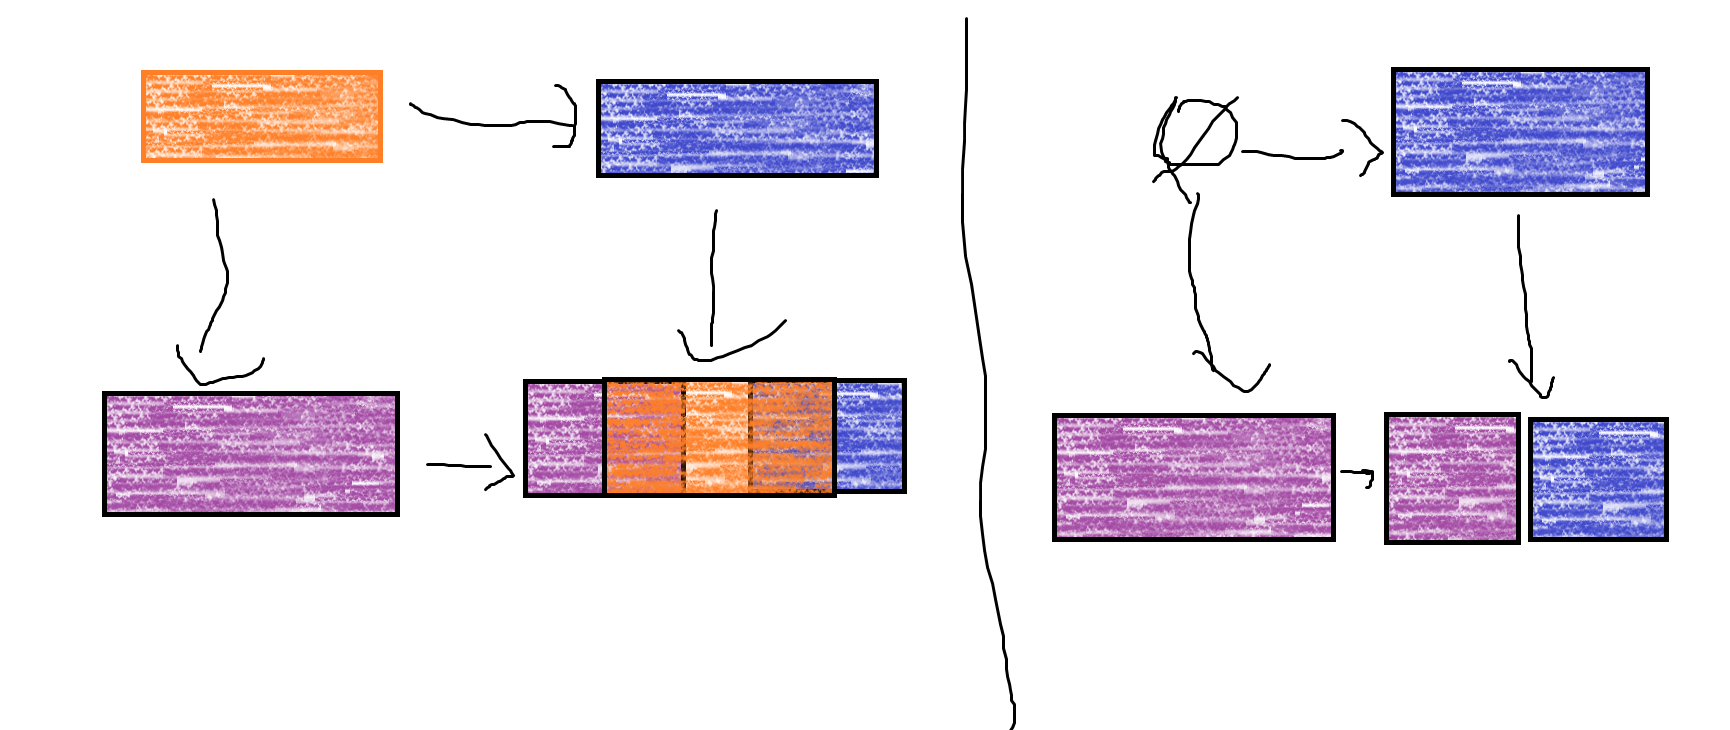
\includegraphics[width=\columnwidth]{k_union.png}
  \label{fig:artist:union:disjoint_k}
  \caption{In \autoref{fig:artist:union:k}, the input object $\sheaf_{\dtotal}$ encodes a continuous function over spaces $\dtotal_a$, $\dtotal_b$ 
  and overlapping space $\dtotal_c$. In this figure, the visual transformation is to a point on the line on screen. An artist that preserves the continuity of the function must generate graphics such that functions evaluated  $\dbasepoint \in \dbase_a \cap \dbase_b$}
\end{figure}

An example of overlapping indexing is a parallelized version of a sliding window algorithm where window overlaps must resolve to the same value at the same position \cite{chuTimeSeriesSegmentation1995}; 


\begin{equation}
\label{eq:artist:intersection:basespace}
\begin{tikzcd}
  \dbasec_{c} \arrow[d, "\iota", hook] \arrow[r, "\iota", hook] & \dbasec_{b} \arrow[d, "i_{\dbasec_b}"]      \\
  \dbasec_{a} \arrow[r, "i_{\dbasec_a}"]                         & \dbasec_{a} \bigsqcup_{\dbasec_{c}}\dbasec_{b}
  \end{tikzcd}
\end{equation}

where the projection functions $i_{\dbase_a},i_{\dbase_b}$ behave such that $i_{\dbase_a}(\dbasepoint)|_{\dbasepoint \in \dbase_b} = \left[\dbasepoint\right]$, $i_{\dbase_b}(\dbasepoint)|_{\dbasepoint \in \dbase_b} = \left[\dbasepoint\right]$, meaning the projection functions yield equivalent points in the disjoint union $\dbase_a \bigsqcup_{\dbase_c} \dbase_b$. Data that is completely disjoint in the index, as shown in \autoref{fig:artist:union:disjoint_k}, is a special case where $\dbase_c=\varnothing$ and therefore there is no constraint on the artist with regards to how this data is rendered. 

\subsubsection{Shared Fields}

\begin{figure}[h!]
  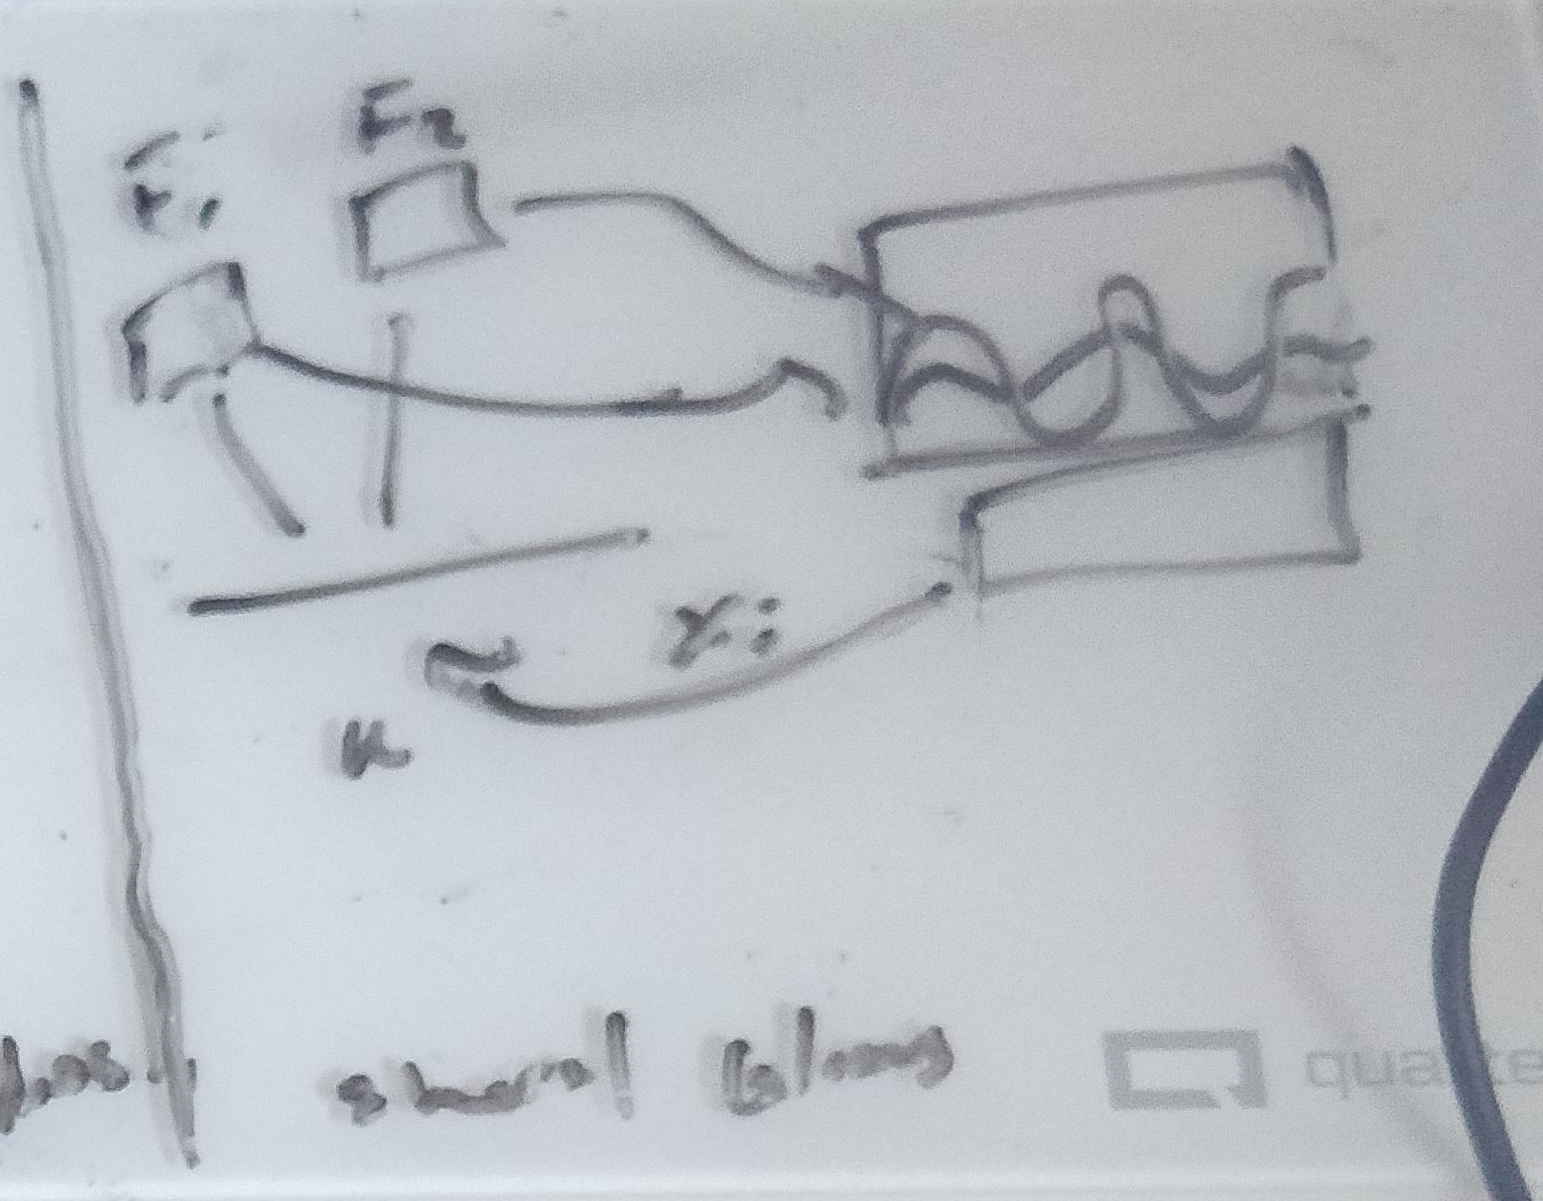
\includegraphics[width=\columnwidth]{intersection_f.png}
  \caption{The fiber spaces $F_a, F_b$ have a shared fiber space $F_c$. If they are input into the same artist $A_1$, then an equivariant transformation is one where $F_c$ is transformed to a visual element in a consistent matter. In this figure, $F_c$ is mapped to the x-axis for both $F_a$ and $F_b$.}
  \label{fig:artist:compose:union_fiber}
\end{figure}

\begin{equation}
  \label{eq:artist:intersection:fiber}
  \begin{tikzcd}
    \dfiberc_{a}\times \dfiberc_{b} \arrow[d, "proj_b"] \arrow[rr, "proj_a"] &  & \dfiberc_{a} \arrow[d, "proj_c"] \\
    \dfiberc_{b} \arrow[rr, "proj_b"]                                                  &  & \dfiberc_{c}                    
    \end{tikzcd}
\end{equation}

\autoref{eq:artist:intersection:basespace} and \autoref{eq:artist:intersection:fiber} can be composed to specify how different aspects of the structure of a multivariate nested dimensional dataset, such as a spatio-temporal weather dataset, should be preserved in a visualization. 
\note{this is probably the power of this model and should maybe get a figure?}


\section{Construction and formal properties of Artists}
\label{sec:artist:construction}
\begin{figure*}[h!]
  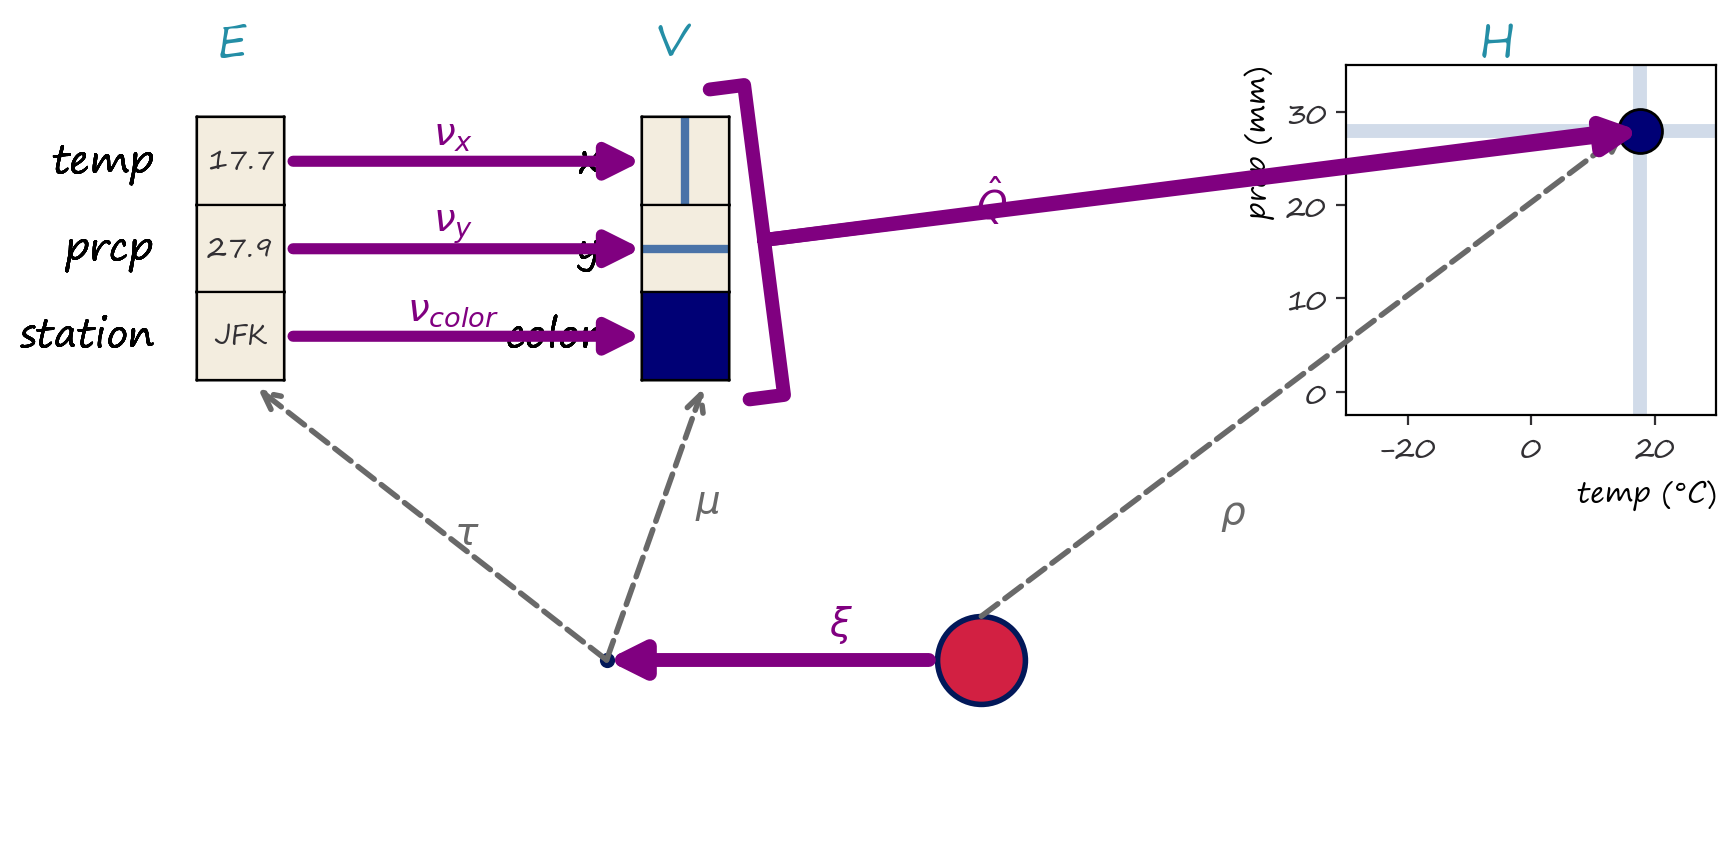
\includegraphics[width=\linewidth]{q.png}
  \caption{}
  \label{fig:constraints:q-overall}
\end{figure*}

Following from \autoref{eq:artist:equivariance}, the artist \vartistc\ is a natural transformation
  \begin{equation}
    \vartist: \sheaf_{\mathcal{\dtotal}}
  \end{equation}
that we construct to preserve continuity and equivariance.

\begin{definition} We define the natural transformation \textcolor{artist}{Artist}  \vartist\ as the tuple $(\vindexc, \vchannelc, \vmarkc, \mathcal{\dtotalc},\mathcal{\vtotalc}, \mathcal{\gtotalc})$ where
  \begin{enumerate}
    \item $\vchannelc: \dtotalc \rightarrow \vtotalc$ is a bundle map from data values to the visual variables they are mapped to
    \item $\vmarkc: \sheafc_{\mathcal{\vtotalc} \rightarrow \sheafc_{\mathcal{\vartistc}}$ is a sheaf map that builds a graphic generating function parameterized by the visual variables 
    \item $\vindexc: \gbasec \rightarrow \dbasec$ is a surjective map from the graphic topological base to the data topological base
  \end{enumerate}
\end{definition}
and $\mathcal{\dtotalc}$, $\mathcal{\vtotalc}$, and $\mathcal{\gtotalc}$ are the categorical representations of fiber bundles that model the data, visual variable, and graphic space of the data to visual transformation.  We construct the artist to have two stages

\begin{equation}
  \label{eq:artist:construction:all}
  \begin{tikzcd}
    \dtotalc \arrow[rr, "\vchannel"] \arrow[rdd, "\pi"'] &         & \dtotalc \arrow[ldd, "\pi"] & \mathcal{\vtotalc}                                                        & Im_{\vmarkc} \subset \gtotalc                     \\
  &         &                             & {} \arrow[r, "\vmarkc"]                                                   & {}                                \\
   & \dbasec &                             & \mathcal{\dbasec} \arrow[uu, "\sheaf_{\vtotalc}"] \arrow[r, "\vindexc^*"] & \mathcal{\gbasec} \arrow[uu, "\sheaf_{\vmarkc}"']
  \end{tikzcd}
\end{equation}
which are the data to visual variable map $\vchannel$ at the bundle level and the visual variable to graphic map $\vmark$ at the sheaf level. Usage of the bundle directly in an equation or diagram - $\dotal, \vtotal, \gtotal$ - denotes that the function can be evaluated pointwise over $\dbasepoint \in \dbase$. Use of the categorical form -- $\mathcal{\dtotalc}, \mathcal{\vtotalc}, \mathcal{\gtotalc}$ -- denotes that the function is evaluated over an openset object, meaning that the function needs knowledge of both a value over a point and some information about neighboring values. 


\subsection{Data Domain}
We model data as sections of a fiber bundle $(\dtotal, \pi, \dbase, \dfiber)$. We encode the continuity of the data as the \textcolor{base}{base space} $\dbase$. \note{does this go in intro?} The \textcolor{fiber}{fiber space} \dfiber\ is the space of all possible values of the data \autoref{eq:related-work:fiber}. We model the data as the section \dsection because, as described in \autoref{sec:related-work:fiber-bundles}, the section is the map from the indexing space \dbase to the space of possible data values \dfiber. Spivak's notation, as discussed in \autoref{sec:related-work:equivariance}, also allows for associating elements in a section with the field it comes from. This allows for field based selection of values, while inclusion allows for continuity (index) based selections. 


\begin{figure}[h!]
  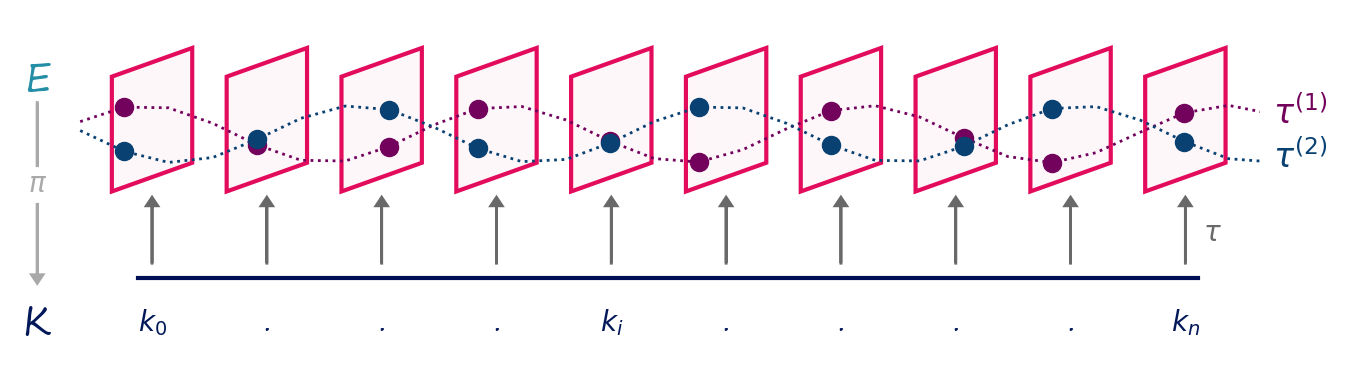
\includegraphics[width=\columnwidth]{fiberbundle.png}
  \caption{\note{replace with more concrete}}
  \label{fig:artist:data}
\end{figure}

One example of encoding data as a section of a fiber bundle is illustrated in \autoref{fig:artist:data}. In this example, the data is a \note{not totally decided yet} table of weather station data. Here we are interested in the time series of temperature values in the data, so we encode the continuity as the 1D interval \dbase. In this multivariate data set, the fields we want to visualize are \texttt{time}, \texttt{temperature}, and \texttt{station}. The fiber space \dfiber\ is the cartesian cross product of the fibers of each field
\begin{equation*}
  \dfiber = \dfiber_{time} \times \dfiber_{temperature} \times \dfiber_{station}
\end{equation*}
where each field fiber is the set of values that are valid for the field: 
\begin{align*}
  \dfiber_{time} &= \mathbb{R} \\
  \dfiber_{temperature} &= \mathbb{R}\\
  \dfiber_{station} &= \{s_0, s_1, \cdots, s_i, \cdots, s_n\} 
\end{align*}

The section \dsection\ is the abstraction of the data being visualized. The section at a point $k \in K$ in the base space returns a value from each field in the fiber.
\begin{equation*}
  \tau(k) = ((time, t_k); (precipitation, p_k); (station\;name, n_k))
\end{equation*}


\subsection{Graphic Codomain} 
The object of the graphic category $\mathcal{\gtotal}$ is the fiber bundle \gtotal. The bundle \gtotal\ has the same structure as the data bundle \dtotal

\begin{equation}
  \begin{tikzcd}[ampersand replacement=\&]
      \gfiber \arrow[r, hook] \& \gtotal \arrow[d, "\pi"'] \\
                        \& \gbase \arrow[u, "\gsection"', bend right]
  \end{tikzcd}
\end{equation}
with a fiber space \gfiber\ embedded in the total space \gtotal\ and a section map $\gsection:\gbase\rightarrow\gtotal$. The attributes of the graphic bundle $(\gtotal, \pi, \gfiber, \gbase)$ encode attributes of the graphic and display space 

\begin{LaTeXdescription}
\item [\textcolor{base}{base space} \gbase] continuity of display space (e.g. screen, 3D print)
\item [\textcolor{fiber}{fiber space} \gfiber] attributes of the display space (e.g a pixel = (x,y,r,g,b,a))
\item [\textcolor{section}{section} \gsection] graphic generating function
\end{LaTeXdescription}.

We represent the graphic output as a fiber bundle because it is an abstraction that is generalizable to various output mediums (screens, 3D prints) and types of graphics.

\begin{figure}[h!]
  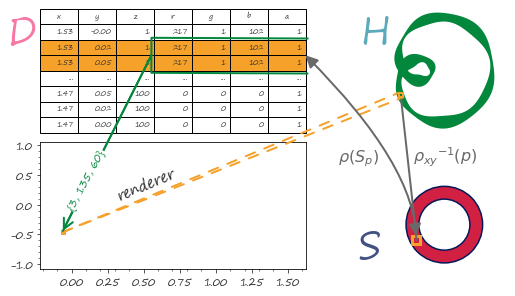
\includegraphics[width=\columnwidth]{render.png}
  \caption{}
  \label{fig:artist:graphic}
\end{figure}

As illustrated in \autoref{fig:artist:graphic}, in this work, \gtotal\ assumes the the display is an idealized 2D screen. \note{include some more about the figure} The graphic section \gsection\ is an abstraction of rendering. For example, \gsection\ can be a specification such as PDF\cite{bienz1993portable}, SVG\cite{quintScalable2003} or an OpenGL scene graph\cite{CarsonOpenGL1997}, or a rendering engine such as Cairo\cite{CairographicsOrg} or AGG\cite{shemanarevAntiGrainGeometry}.

\subsection{Visualization Library Components}


\subsubsection{Visual Bundle \vtotal}
\begin{equation}
  \begin{tikzcd}[ampersand replacement=\&]
      \vfiber \arrow[r, hook] \& \vtotal \arrow[d, "\pi"'] \\
                        \& \dbase \arrow[u, "\vsection"', bend right]
  \end{tikzcd}
\end{equation}

\subsubsection{Graphic to Data: \vindex}
\begin{equation}
  \label{eq:artist:construction:xi}
  \begin{tikzcd}
      \dtotal \arrow[d, "\pi"'] & \gtotal \arrow[d, "\pi"'] \\
      \dbase                   & \gbase \arrow[l, "\vindex"']
  \end{tikzcd}
\end{equation}

The functor $\vindex$ is a deformation retract, which means....\cite{hatcherAlgebraicTopology2002,spanier1989algebraic}


\begin{figure}[!h]
  \centering
  \subfloat[\dbasec_a \sqcup_{\dbasec_c} \dbase_b]{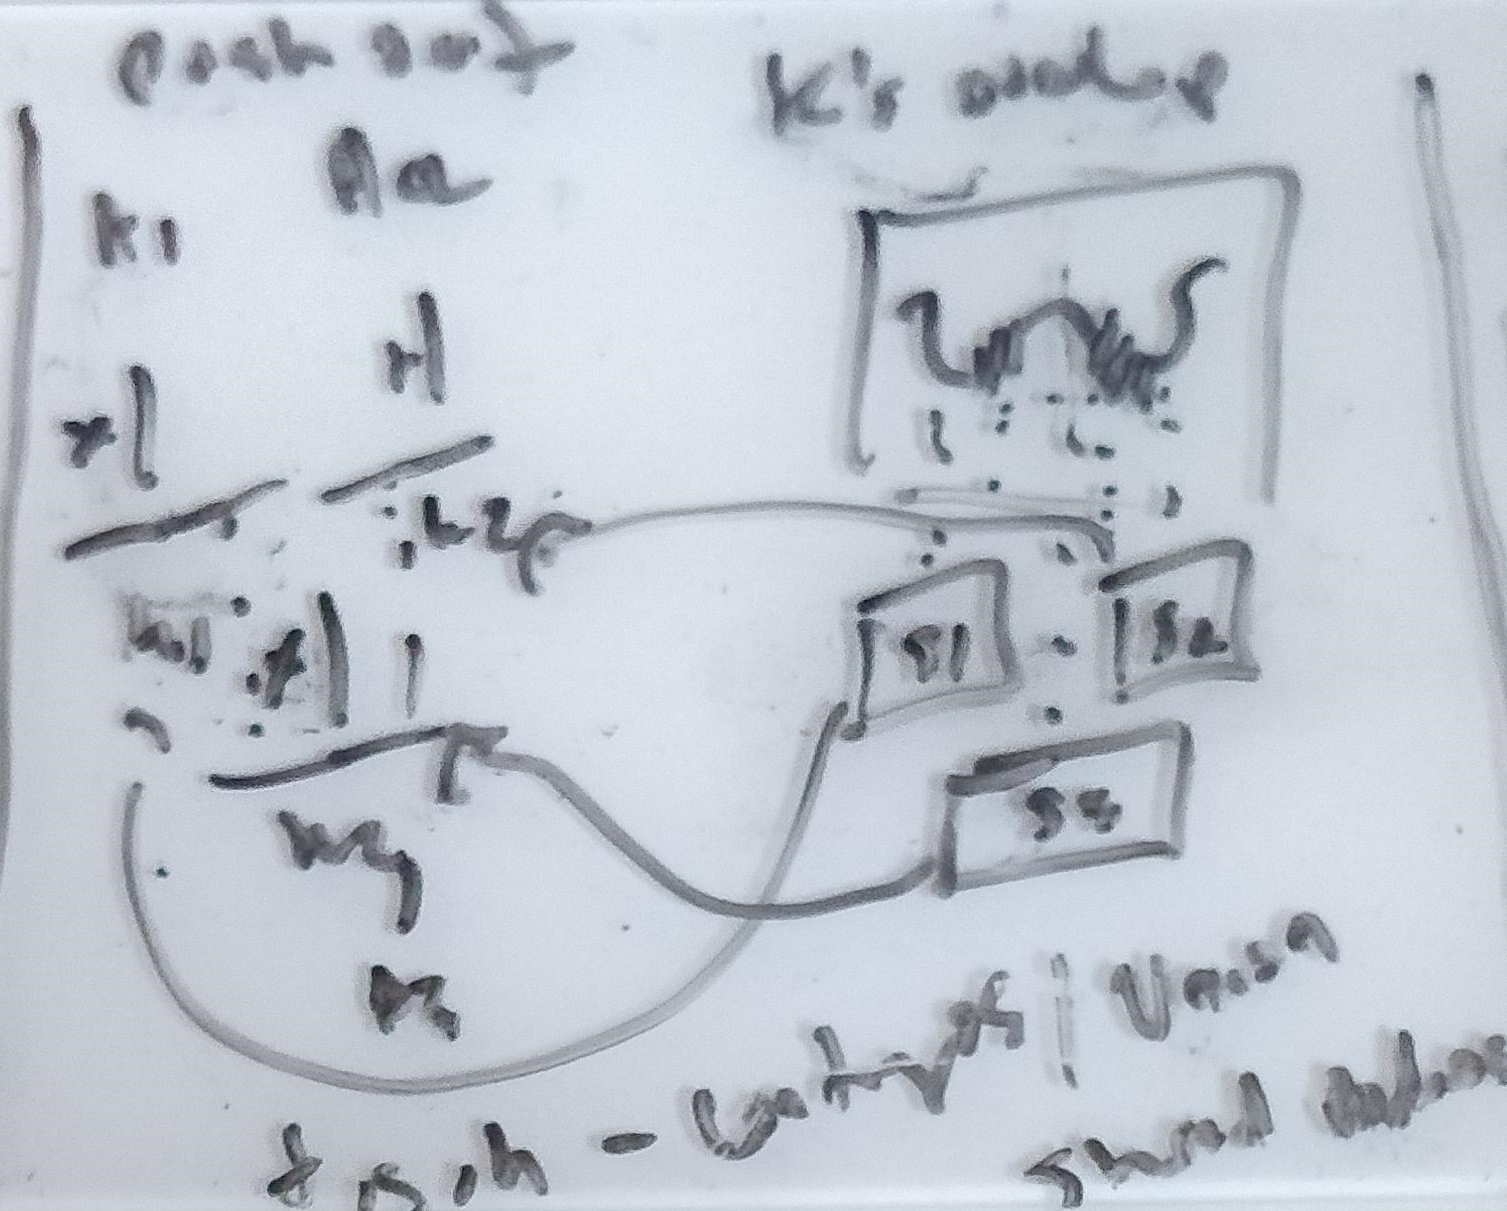
\includegraphics[width=1.2in]{union_k.png}%
  \label{fig_first_case}}
  %\hfil
  \subfloat[\dbasec_c=\varnothing]{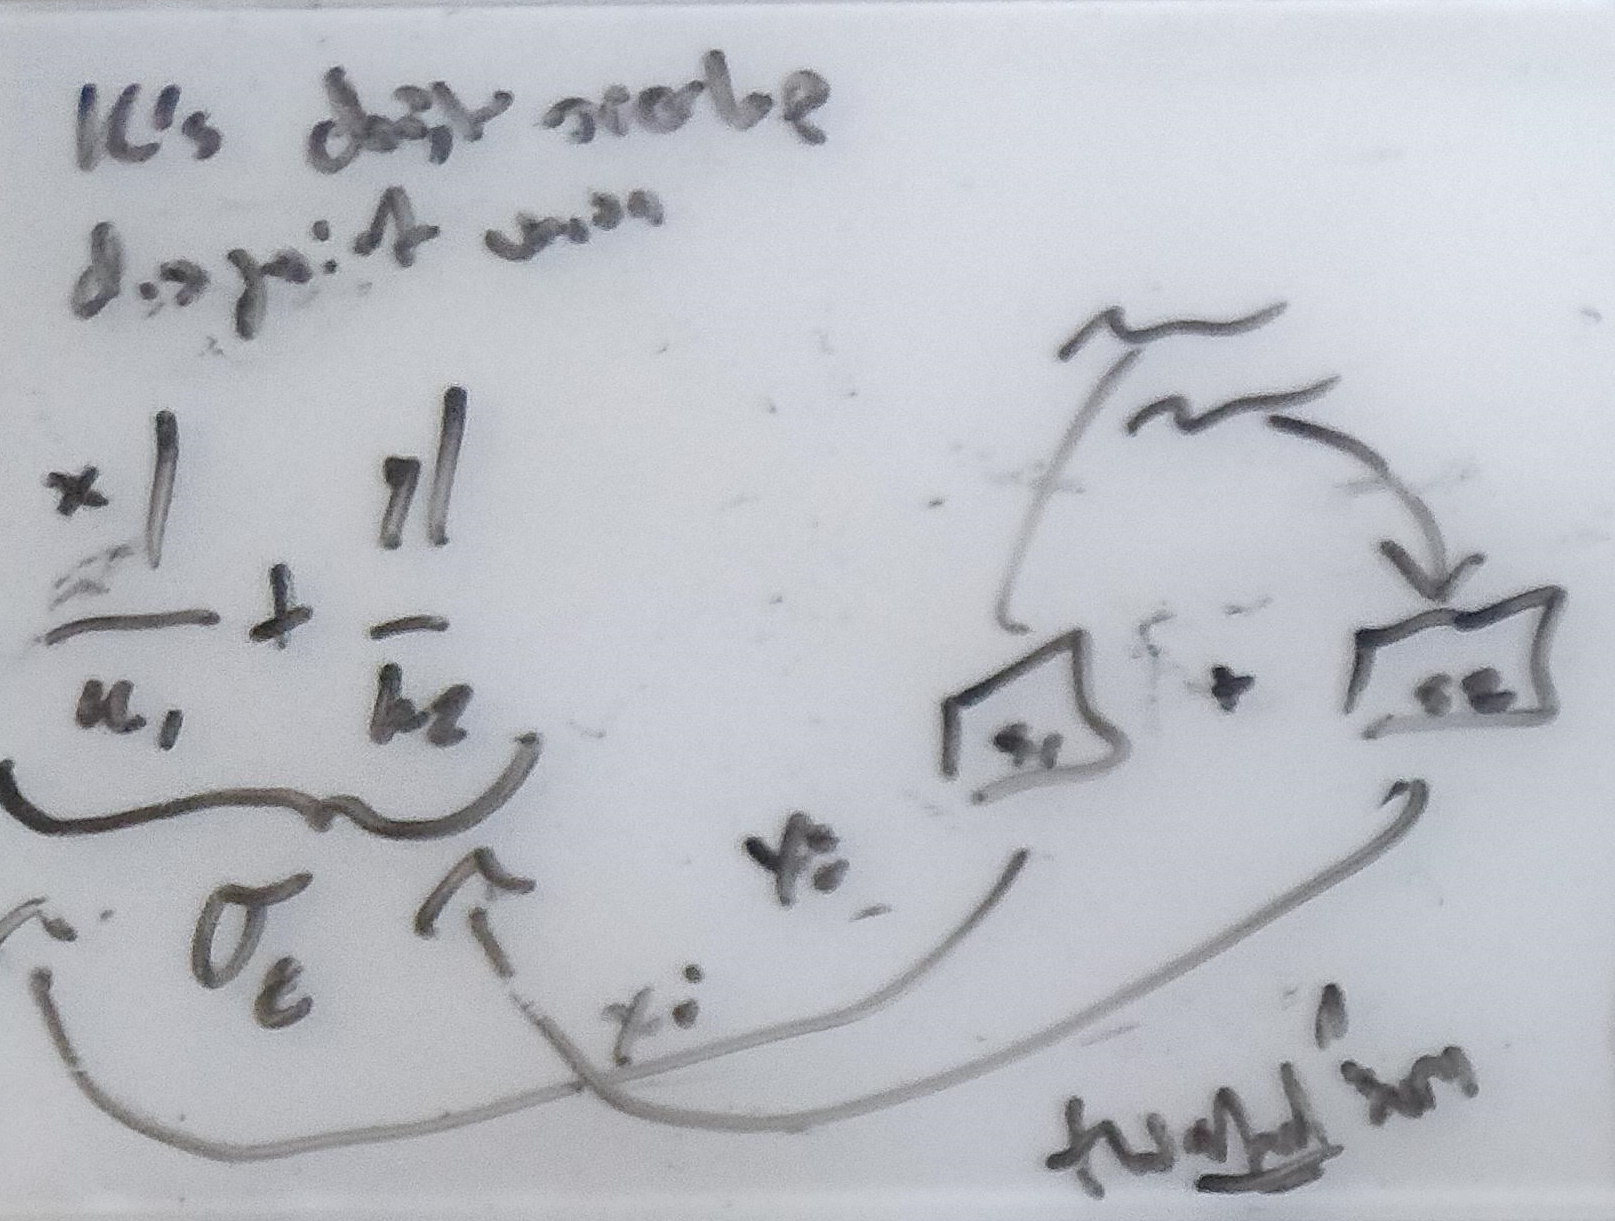
\includegraphics[width=1.2in]{disjoint_k.png}%
  \label{fig_second_case}}
  \caption{\note{probably doesn't need the k=0}}
  \label{fig_sim}
\end{figure}

\begin{equation}
  \label{eq:artist:construction:xi:multi_base}
  \begin{tikzcd}
    \dbase_{c} \arrow[d, hook] \arrow[r, hook] & \dbase_{b}                 & \gbase_b \arrow[l, "\vindex"]                                                \\
    \dbase_{a}                                 & \gbase_a \arrow[l, "\vindex"'] & \gbase_c \arrow[l, hook'] \arrow[u, hook] \arrow[llu, "\vindex" description]
  \end{tikzcd}
\end{equation}

Can be implemented in V

\begin{equation}
  \label{eq:artist:construction:xi:v}
  \begin{tikzcd}
  \textcolor{color=gray!50}{\dtotal}\arrow[rd, "\pi"', color=gray!50] & \vtotal \arrow[d, "\pi"] & \vindex^*\vtotal \arrow[d, "\vindex^*\pi"'] \arrow[l, "\vindex^*"', dashed] & \textcolor{color=gray!50}{\gtotal} \arrow[ld, "\pi", color=gray!50] \\
    & \dbase                   & \gbase \arrow[l, "\vindex"']                                                &                          
    \end{tikzcd}
\end{equation}

\subsubsection{Data to Visual Encodings: \vchannel} 
\begin{equation}
  \label{eq:artist:construction:nu}
\begin{tikzcd}
  \dtotal \arrow[rd, "\pi"'] \arrow[r, "\vchannel"] & \vtotal \arrow[d, "\pi"] & \textcolor{fade}{\vindex^*\vtotal} \arrow[d, "\vindex^*\pi"', color=fade] \arrow[l, "\vindex^*", color=fade] & \textcolor{fade}{\gtotal} \arrow[ld, "\pi", color=fade] \\
& \dbase                   & \textcolor{gray!50}{\gbase} \arrow[l, "\vindex"', color=gray!50]                                       &                          
  \end{tikzcd}
\end{equation}

Visual encoding functions \vindex\ are functors because they are expected to preserve structure on the data and visual side, as discussed in \autoref{sec:related-work:equivariance}. 

 This constraint is expressed in our construction of \vchannel

\begin{figure}[!h]
  \centering
  \subfloat[Artists with shared $\mu_i$ renderered correctly]{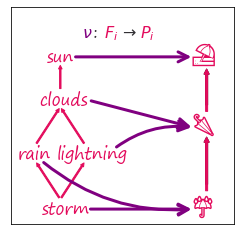
\includegraphics[width=1.2in]{partial_fixed.png}%
  \label{fig_first_case}}
  %\hfil
  \subfloat[Artists without shared $\mu_i$]{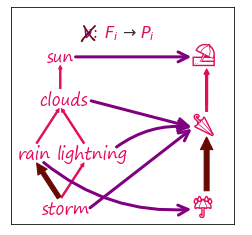
\includegraphics[width=1.2in]{partial_invalid.png}%
  \label{fig_second_case}}
  \caption{Simulation results for the network.}
  \label{fig_sim}
  \end{figure}


\begin{equation}
\label{eq:artist:construction:nu:fiber_map}
\begin{tikzcd}[column sep=.5em]
  \dfiber \arrow[rr, "\vchannel"] &                                                         & \vfiber \\
                                  & \dbase \arrow[lu, "\dsection"] \arrow[ru, "\vsection"'] &        
  \end{tikzcd}
\end{equation}

which means equivariance of 
\begin{equation}
\label{eq:artist:construction:nu:equivariance}
\begin{tikzcd}
  \dsection \arrow[d, "\varphi"'] \arrow[r, "\vchannel"] & \vsection \arrow[d, "\vchannel_{\varphi}"] \\
  \dsection^{\prime} \arrow[r, "\vchannel"]                       & \vsection^{\prime}                                 
  \end{tikzcd}
\end{equation}

\paragraph{Multiview Constraints}
\begin{figure}[!h]
  \centering
  \subfloat[No shared fields]]{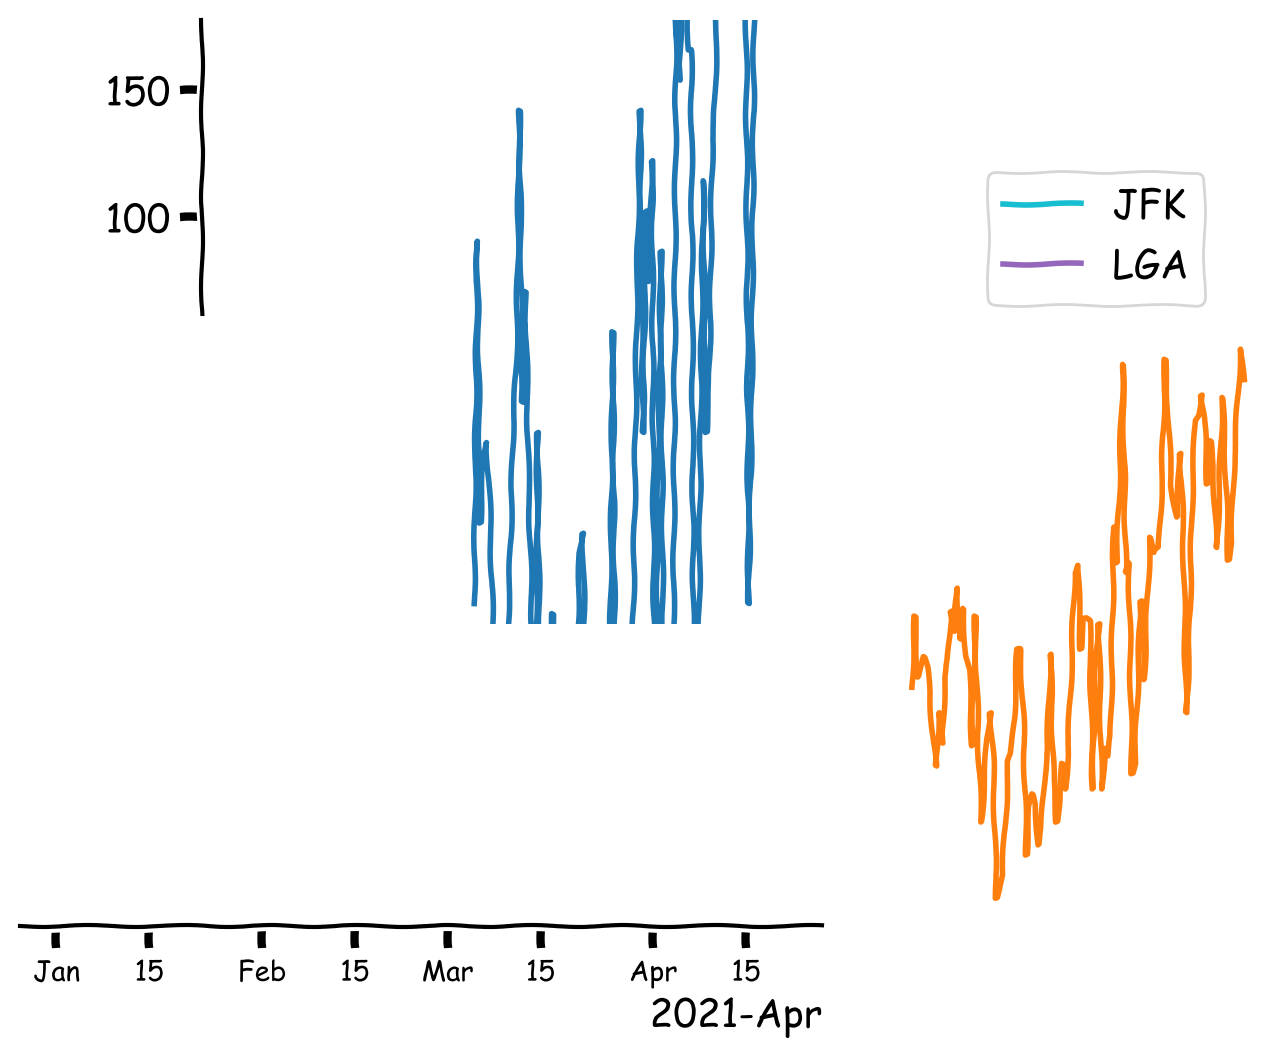
\includegraphics[width=.4\columnwidth]{exploding_artist.png}%
  \label{fig:artist:union:k}}
  %\hfill
  \subfloat[Shared fields]{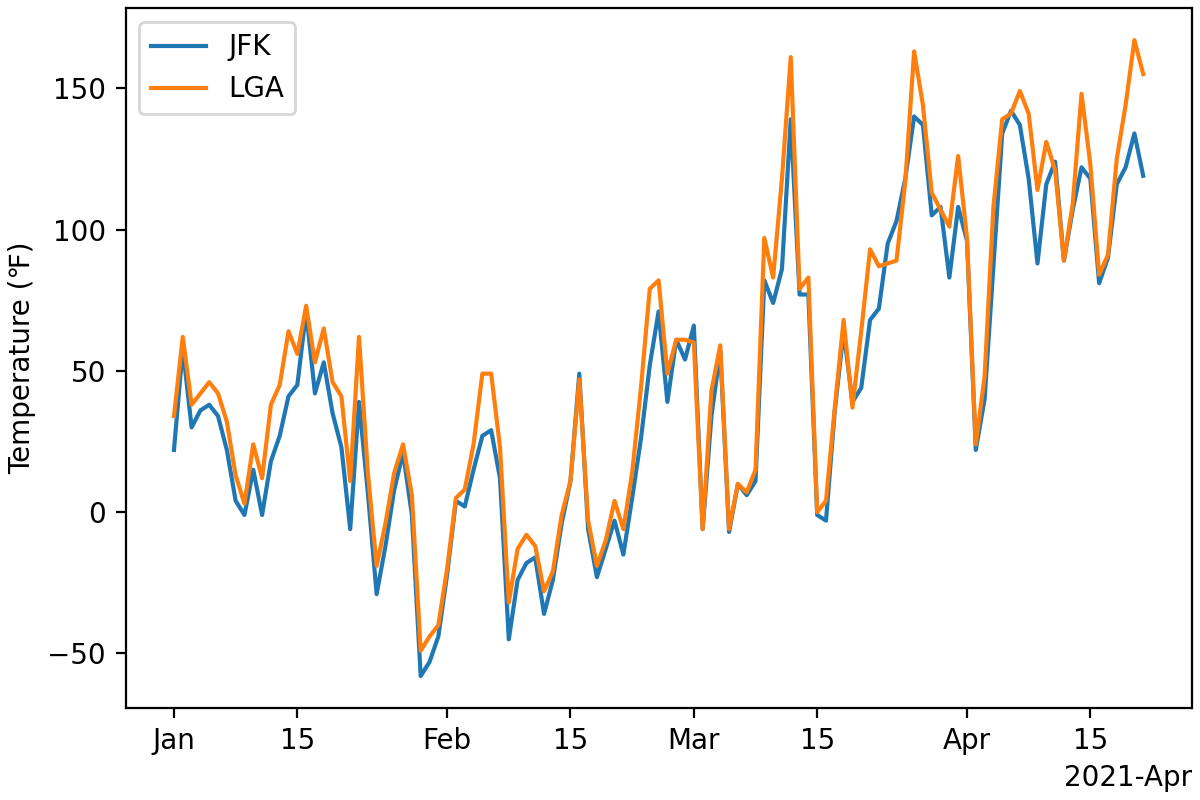
\includegraphics[width=.4\columnwidth]{combined_artist.png}%
  \label{fig:artist:union:disjoint_k}}
  \caption{In \autoref{fig:artist:union:k}, the input object $\sheaf_{\dtotal}$ encodes a continuous function over spaces $\dtotal_a$, $\dtotal_b$ 
  and overlapping space $\dtotal_c$. In this figure, the visual transformation is to a point on the line on screen. An artist that preserves the continuity of the function must generate graphics such that functions evaluted  $\dbasepoint \in \dbase_a \cap \dbase_b$
  \note{replace a) w/ fiber cross diagram? - use first half introduced in \autoref{fig:artist:compose:union_fiber}}}
\end{figure}

The concept that shared data fields should be encoded visually in a consistent is formally expressed by Qu and Hullman \cite{hullmanKeeping2018} as the notion that the same field should have the same scale. 



\begin{equation}
  \label{eq:math:artist:nu}
  \{\vchannel_{0}, \ldots, \vchannel_{n}\}: \{\dsection_{0}, \ldots, \dsection_{n}\} \mapsto \{\vsection_{0}, \ldots, \vsection_{n}\}
\end{equation}

We enforce the equivariance constraint specified in \autoref{eq:artist:construction:multi_nu} by constructing artists that apply \vchannel\ encoders such that 
\begin{equation}
  \label{eq:artist:construction:multi_nu}
  \begin{tikzcd}[row sep=.5em]
    \dfiberc_a \arrow[rrd, "proj_a" description] \arrow[rrrr, "\vchannelc_c"]  &  &  &  & \vfiberc_c \\
    &  & \dfiberc_{c} \arrow[rru, "\vchannelc_c" description] \arrow[rrd, "\vchannelc^{\prime}_c" description] &  & \\
    \dfiberc_b \arrow[rru, "proj_b" description] \arrow[rrrr, "{\vchannelc_c}^{\prime}"'] &  &                                                                                                       &  & {\vfiberc_c}^{\prime}
    \end{tikzcd}
\end{equation}

\subsubsection{Visual to Graphic: \vmark} 
\begin{equation}
  \label{eq:artist:construction:q}
  \begin{tikzcd}
    \textcolor{fade}{\dtotal} \arrow[rd, "\pi"', color=fade] \arrow[r, "\vchannel", color=fade] & \textcolor{gray!50}{\vtotal} \arrow[d, "\pi", color=fade] & \vindex^*\vtotal \arrow[d, "\vindex^*\pi"'] \arrow[l, "\vindex^*"', color=fade] \arrow[r, "\vmark"] & \gtotal \arrow[ld, "\pi"] \\
    & \textcolor{fade}{\dbase} & \gbase \arrow[l, "\vindex"', color=fade]                                            &                          
    \end{tikzcd}
\end{equation}

\begin{equation}
  \label{eq:artist:construction:q:xi}
  \begin{tikzcd}
    \vtotalc \arrow[rr, "\vmarkdc", bend left] & \vtotalpullc \arrow[l, "\vindexc^*"] \arrow[r, "\vmarkc"'] & \gtotalc
  \end{tikzcd}
\end{equation}

\begin{equation}
  \label{eq:artist:construction:q:fiber}
  \begin{tikzcd}[column sep=.5em]
    \vfiber \arrow[rr, "\vmark"] &                                                         & \gfiber \\
    & \gbase \arrow[ru, "\gsection"'] \arrow[lu, "\vsection"] &        
    \end{tikzcd}
\end{equation}
Visual encodings to something like marks 


\begin{equation}
  \label{eq:artist:construction:q:equivariance}
  \begin{tikzcd}
    \vsection \arrow[d, "\vchannel_\varphi"'] \arrow[r, "\vmark"] & \gsection \arrow[d, "\vmark_\varphi"] \\
    \vsection^{\prime} \arrow[r, "\vmark"]                                 & \gsection^{\prime}                            
    \end{tikzcd}
\end{equation}

\begin{figure}[!h]
  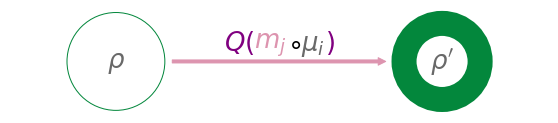
\includegraphics[width=\columnwidth]{diff_type_q.png}
  \caption{rework this as a commutative box w/ the r in E row associated w/ this qhat(k)}
\end{figure}

\begin{equation}
  \label{eq:artist:construction:q:multifiber}
\begin{tikzcd}
  \dfiberc_a \arrow[rr, "\vchannelc"] \arrow[rd, "proj_a" description]          &            & \vfiberc_a \arrow[rr, "\vmarkd"]         &  & Im_{\vmarkdc} \subset \gtotalc \arrow[llld, "g_a" description, dashed]                  \\
 & \dfiberc_c &                                          &  &\\
  \dfiberc_b \arrow[rr, "\vchannelc^{\prime}"] \arrow[ru, "proj_b" description] &            & \vfiberc_b \arrow[rr, "\vmarkd^{\prime}"] &  & Im_{\vmarkdc^{\prime}}\subset \gtotalc^{\prime} \arrow[lllu, "g_b" description, dashed]
  \end{tikzcd}
\end{equation}

\section{Case Study}
\label{sec:case-study}
\begin{figure}[h!]
  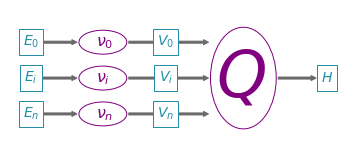
\includegraphics[width=\columnwidth]{path_of_q.png}
    \caption{\note{add in xi!}}
  \label{fig:api}
\end{figure}
We implement the \textbf{arrows} in \autoref{fig:api}. \mintinline{python}{axesArtist} is a parent artist that acts as a screen. This allows for the composition described in                                           \autoref{sec:artist:union}

\subsection{\vartist}
\begin{minted}{python}
for local_tau in axesArtist.artist.data.query(screen_bounds, dpi):
    mu = axesArtist.artist.graphic.mu(local_tau)
    rho = axesArtist.artist.graphic.qhat(**mu)
    H = rho(renderer)
\end{minted}

where the artist is already parameterized with the \vindex\ functions and which fibers they are associated to:

\begin{minted}{python}
\end{minted}


\subsubsection{\vindex}
\subsubsection{\vchannel}
\subsubsection{\vmarkd}



\section{Discussion}
\subsection{Limitations}
\subsection{future work}

\section{Conclusion}
The conclusion goes here.


\appendices




% use section* for acknowledgment
\ifCLASSOPTIONcompsoc
  % The Computer Society usually uses the plural form
  \section*{Acknowledgments}
\else
  % regular IEEE prefers the singular form
  \section*{Acknowledgment}
\fi


The authors would like to thank...


% Can use something like this to put references on a page
% by themselves when using endfloat and the captionsoff option.
\ifCLASSOPTIONcaptionsoff
  \newpage
\fi

% trigger a \newpage just before the given reference
% number - used to balance the columns on the last page
% adjust value as needed - may need to be readjusted if
% the document is modified later
%\IEEEtriggeratref{8}
% The "triggered" command can be changed if desired:
%\IEEEtriggercmd{\enlargethispage{-5in}}

% references section

% can use a bibliography generated by BibTeX as a .bbl file
% BibTeX documentation can be easily obtained at:
% http://mirror.ctan.org/biblio/bibtex/contrib/doc/
% The IEEEtran BibTeX style support page is at:
% http://www.michaelshell.org/tex/ieeetran/bibtex/
\bibliographystyle{IEEEtran}
% argument is your BibTeX string definitions and bibliography database(s)
\bibliography{bibliography}

% biography section 
% If you have an EPS/PDF photo (graphicx package needed) extra braces are
% needed around the contents of the optional argument to biography to prevent
% the LaTeX parser from getting confused when it sees the complicated
% \includegraphics command within an optional argument. (You could create
% your own custom macro containing the \includegraphics command to make things
% simpler here.)
%\begin{IEEEbiography}[{\includegraphics[width=1in,height=1.25in,clip,keepaspectratio]{mshell}}]{Michael Shell}
% or if you just want to reserve a space for a photo:

%\begin{IEEEbiography}{Michael Shell}
%\end{IEEEbiography}

% if you will not have a photo at all:
\begin{IEEEbiographynophoto}{Hannah Aizenman}
Biography text here.
\end{IEEEbiographynophoto}

\begin{IEEEbiographynophoto}{Thomas Caswell}
  Biography text here.
\end{IEEEbiographynophoto}
% insert where needed to balance the two columns on the last page with
% biographies
%\newpage

\begin{IEEEbiographynophoto}{Michael Grossberg}
Biography text here.
\end{IEEEbiographynophoto}

% You can push biographies down or up by placing
% a \vfill before or after them. The appropriate
% use of \vfill depends on what kind of text is
% on the last page and whether or not the columns
% are being equalized.

%\vfill

% Can be used to pull up biographies so that the bottom of the last one
% is flush with the other column.
%\enlargethispage{-5in}

% that's all folks
\end{document}


